\documentclass[twocolumn,10pt,a4paper]{article}

% Page layout
\usepackage[margin=2cm, columnsep=0.6cm]{geometry}
\usepackage[utf8]{inputenc}
\usepackage[T1]{fontenc}

% Packages
\usepackage{amsmath,amssymb,amsthm}
\usepackage{mathtools}
\usepackage{physics}
\usepackage{bm}
\usepackage{graphicx}
\usepackage{hyperref}
\usepackage{cleveref}
\usepackage{enumitem}
\usepackage{booktabs}
\usepackage{multirow}
\usepackage{algorithm}
\usepackage{algpseudocode}
\usepackage{natbib}
\usepackage{xcolor}

% Theorem environments
\newtheorem{theorem}{Theorem}[section]
\newtheorem{lemma}[theorem]{Lemma}
\newtheorem{proposition}[theorem]{Proposition}
\newtheorem{corollary}[theorem]{Corollary}
\newtheorem{definition}[theorem]{Definition}
\newtheorem{axiom}{Axiom}
\newtheorem{remark}[theorem]{Remark}

% Custom commands
\newcommand{\Sspace}{\mathcal{S}}
\newcommand{\Sk}{S_k}
\newcommand{\St}{S_t}
\newcommand{\Se}{S_e}
\newcommand{\trit}{\mathfrak{t}}
\newcommand{\R}{\mathbb{R}}
\newcommand{\N}{\mathbb{N}}
\newcommand{\Z}{\mathbb{Z}}
\newcommand{\C}{\mathbb{C}}
\newcommand{\kB}{k_{\text{B}}}
\newcommand{\Mpart}{M_{\text{part}}}

\title{Trajectory Completion Cheminformatics: \\
A Dynamical Systems Framework for Molecular Identification \\
via Penultimate State Analysis in Entropy Coordinate Space}

\author{
    Kundai Farai Sachikonye\\
    \texttt{kundai.sachikonye@wzw.tum.de}
}


\date{\today}

\begin{document}

\maketitle

\begin{abstract}
We present a reformulation of cheminformatics as a problem in dynamical systems theory, wherein molecular identification corresponds to trajectory completion in a bounded phase space. Starting from the single axiom that physical systems occupy finite domains, we derive that bounded continuous dynamics necessarily exhibit oscillatory behavior (via Poincar\'{e} recurrence), which induces categorical state structure, which in turn defines partition operations on phase space. These three descriptions---oscillatory, categorical, and partitional---are shown to be mathematically equivalent, related by canonical isomorphisms. We construct an entropy coordinate space $\Sspace = [0,1]^3$ with coordinates encoding kinetic configuration, temporal structure, and evolutionary depth. Molecular species correspond to fixed points in $\Sspace$, and molecular identification reduces to trajectory convergence toward these attractors. We introduce the concept of \emph{penultimate states}---the pre-images of fixed points under the dynamics---which provide actionable targets for identification algorithms. A ternary encoding scheme maps molecular structures to addresses in $\Sspace$, where the address simultaneously specifies position and the trajectory leading to that position. We demonstrate that this framework achieves categorical temporal resolution exceeding Planck-scale limits through phase accumulation mechanisms, enabling discrimination between arbitrarily similar molecular species. The theory transforms cheminformatics from a pattern-matching discipline into a branch of ergodic theory, with molecular databases reconceptualized as atlases of dynamical fixed points. We provide rigorous proofs for all major results and discuss implications for spectroscopic measurement theory.
\end{abstract}

\section{Introduction}

Contemporary cheminformatics treats molecular identification as a pattern recognition problem \citep{todeschini2009molecular}. Given a set of molecular descriptors---computed properties, fingerprints, spectroscopic signatures---the task is to match an unknown sample against a database of known species. This formulation, while practically successful, lacks a principled theoretical foundation. Why should molecules be identifiable at all? What mathematical structure guarantees that distinct species produce distinguishable signatures? What are the fundamental limits of molecular discrimination?

This paper develops an alternative formulation grounded in dynamical systems theory. We show that molecular identification is not fundamentally a pattern-matching problem but rather a \emph{trajectory completion} problem in phase space. The key insight is that physical systems occupying bounded domains must exhibit recurrent dynamics \citep{poincare1890probleme}, which induces a natural categorical structure on trajectories. Molecules correspond to fixed points---attractors---in this categorical space, and identification consists of determining which fixed point a given trajectory approaches.

The reformulation offers several advantages. First, it provides a mathematical proof that molecular identification is always possible in principle: the categorical structure induced by bounded dynamics guarantees distinguishability. Second, it reveals the geometric structure underlying spectroscopic measurement: spectrometers do not extract pre-existing information but rather implement specific couplings that probe categorical state transitions. Third, it suggests new computational architectures wherein hardware oscillators serve as physical spectrometers, not simulations thereof.

The paper is organized as follows. Section~\ref{sec:axiom} introduces the foundational axiom of bounded phase space. Section~\ref{sec:oscillation} proves that bounded continuous dynamics necessarily exhibit oscillatory behavior. Section~\ref{sec:categories} shows how oscillation induces categorical state structure. Section~\ref{sec:partitions} establishes the equivalence between categorical states and partition operations. Section~\ref{sec:triple} proves the Triple Equivalence Theorem unifying these three descriptions. Section~\ref{sec:entropy_space} constructs the entropy coordinate space. Section~\ref{sec:ternary} develops ternary encoding for three-dimensional spaces. Section~\ref{sec:fixed_points} characterizes molecules as fixed points. Section~\ref{sec:penultimate} introduces penultimate state analysis. Section~\ref{sec:encoder} presents the molecular encoder algorithm. Section~\ref{sec:trans_planckian} analyzes categorical temporal resolution. Section~\ref{sec:applications} discusses applications and implications.

\section{The Bounded Phase Space Axiom}
\label{sec:axiom}

We begin with a single foundational principle from which all subsequent results derive.

\begin{axiom}[Bounded Phase Space]
\label{ax:bounded}
Every physical system occupies a phase space $M$ of finite measure: $\mu(M) < \infty$ for some appropriate measure $\mu$.
\end{axiom}

This axiom is not an arbitrary postulate but reflects fundamental physical constraints. Thermodynamically, systems with unbounded phase space would have infinite entropy, violating the third law \citep{nernst1906warmesatz}. Quantum mechanically, phase space volumes are quantized in units of $h^{3N}$ for $N$ degrees of freedom, where $h$ is Planck's constant \citep{planck1901gesetz}. General relativistically, horizons bound causally accessible regions \citep{bekenstein1973black}. The axiom captures the common content of these diverse physical principles.

\begin{definition}[Bounded Dynamical System]
A dynamical system $(M, \phi_t, \mu)$ is \emph{bounded} if:
\begin{enumerate}[label=(\roman*)]
    \item The phase space $M$ is a measurable set with $\mu(M) < \infty$
    \item The flow $\phi_t: M \to M$ is measurable for all $t \in \R$
    \item The measure $\mu$ is invariant under the flow: $\mu(\phi_t(A)) = \mu(A)$ for all measurable $A \subseteq M$
\end{enumerate}
\end{definition}

The requirement of measure-preserving dynamics follows from Liouville's theorem for Hamiltonian systems \citep{liouville1838note} and its generalizations to broader classes of physical dynamics \citep{arnold1989mathematical}.

\section{Oscillatory Necessity for Bounded Dynamics}
\label{sec:oscillation}

The first major consequence of bounded phase space is that trajectories must return arbitrarily close to their starting points---they cannot escape to infinity or explore ever-new regions indefinitely.

\begin{theorem}[Poincar\'{e} Recurrence]
\label{thm:poincare}
For a bounded measure-preserving dynamical system $(M, \phi_t, \mu)$ and any measurable set $A \subset M$ with $\mu(A) > 0$, almost every point $x \in A$ returns to $A$ infinitely often. Formally, for $\mu$-almost every $x \in A$, the set $\{t > 0 : \phi_t(x) \in A\}$ is unbounded.
\end{theorem}

\begin{proof}
Define the non-returning set at time $n$:
\begin{equation}
A_n = \{x \in A : \phi_t(x) \notin A \text{ for all } t > n\}
\end{equation}
These sets are nested: $A_1 \supseteq A_2 \supseteq A_3 \supseteq \cdots$. Let $A_\infty = \bigcap_{n=1}^\infty A_n$ be the set of points that never return after some finite time.

For fixed $n$, consider the sequence of sets $A_\infty, \phi_n(A_\infty), \phi_{2n}(A_\infty), \ldots$ These are pairwise disjoint: if $\phi_{jn}(x) = \phi_{kn}(y)$ for $x, y \in A_\infty$ with $j < k$, then $\phi_{(k-j)n}(y) = x \in A$, contradicting $y \in A_\infty$.

Since $\mu$ is $\phi_t$-invariant, $\mu(\phi_{kn}(A_\infty)) = \mu(A_\infty)$ for all $k \geq 0$. If $\mu(A_\infty) > 0$, then:
\begin{equation}
\mu(M) \geq \sum_{k=0}^\infty \mu(\phi_{kn}(A_\infty)) = \sum_{k=0}^\infty \mu(A_\infty) = \infty
\end{equation}
contradicting $\mu(M) < \infty$. Therefore $\mu(A_\infty) = 0$, proving almost every point returns infinitely often.
\end{proof}

This classical result, due to Poincar\'{e} \citep{poincare1890probleme}, has profound implications. In bounded systems, trajectories are necessarily recurrent---they revisit neighborhoods of their initial conditions repeatedly.

\begin{theorem}[Oscillatory Necessity]
\label{thm:oscillation}
Let $(M, \phi_t)$ be a bounded continuous dynamical system with $M \subset \R^n$ compact. For almost every initial condition $x_0 \in M$, the trajectory $\{\phi_t(x_0)\}_{t \geq 0}$ exhibits recurrent behavior. For systems with smooth flow, recurrence manifests as oscillation around periodic orbits or equilibrium points.
\end{theorem}

\begin{proof}
By compactness of $M$, the trajectory $\gamma(x_0) = \overline{\{\phi_t(x_0) : t \geq 0\}}$ has compact closure. By Theorem~\ref{thm:poincare}, almost every $x_0$ returns arbitrarily close to itself.

Define the return time function for $\epsilon > 0$:
\begin{equation}
T_\epsilon(x) = \inf\{t > 0 : d(\phi_t(x), x) < \epsilon\}
\end{equation}
where $d$ is the metric on $M$. By Poincar\'{e} recurrence, $T_\epsilon(x) < \infty$ for almost every $x$ and every $\epsilon > 0$.

For smooth flows on compact manifolds, the Poincar\'{e}-Bendixson theory \citep{poincare1881memoire, bendixson1901courbes} implies that recurrent trajectories either converge to equilibria, periodic orbits, or quasi-periodic motion on tori. In all cases, the dynamics are oscillatory in the sense that the trajectory repeatedly traverses similar regions of phase space.

Specifically, consider the closure $\omega(x_0) = \bigcap_{T>0} \overline{\{\phi_t(x_0) : t > T\}}$ (the $\omega$-limit set). For bounded systems with smooth flow, $\omega(x_0)$ is non-empty, compact, connected, and invariant. The restriction of $\phi_t$ to $\omega(x_0)$ exhibits periodic or quasi-periodic motion \citep{smale1967differentiable}, which constitutes oscillatory behavior.
\end{proof}

\begin{remark}
The oscillatory necessity theorem transforms a topological constraint (boundedness) into a dynamical constraint (recurrence/oscillation). This is the first step in our derivation: bounded phase space $\Rightarrow$ oscillatory dynamics.
\end{remark}

\section{Categorical State Structure from Oscillation}
\label{sec:categories}

Oscillatory dynamics with characteristic period $T$ induce a natural partition of time into categorical states---complete cycles of oscillation.

\begin{definition}[Categorical States]
\label{def:categorical}
For an oscillatory system with period $T > 0$, the \emph{categorical state} at time $t$ is:
\begin{equation}
\mathcal{C}(t) = \lfloor t/T \rfloor \in \Z
\end{equation}
The categorical state counts complete oscillation cycles elapsed since $t = 0$.
\end{definition}

\begin{definition}[Categorical Partition of Time]
The categorical state function induces a partition of the time axis:
\begin{equation}
\mathcal{C}_n = \{t \in \R : nT \leq t < (n+1)T\} = [nT, (n+1)T)
\end{equation}
for $n \in \Z$.
\end{definition}

\begin{theorem}[Categorical Structure Theorem]
\label{thm:categorical}
The partition $\{\mathcal{C}_n\}_{n \in \Z}$ satisfies:
\begin{enumerate}[label=(\roman*)]
    \item \textbf{Completeness:} $\bigcup_{n \in \Z} \mathcal{C}_n = \R$
    \item \textbf{Disjointness:} $\mathcal{C}_n \cap \mathcal{C}_m = \emptyset$ for $n \neq m$
    \item \textbf{Translation covariance:} $\mathcal{C}_{n+k} = \mathcal{C}_n + kT$
    \item \textbf{Countable cardinality:} $|\{\mathcal{C}_n : n \in \Z\}| = \aleph_0$
\end{enumerate}
\end{theorem}

\begin{proof}
(i) For any $t \in \R$, define $n = \lfloor t/T \rfloor$. Then $nT \leq t < (n+1)T$, so $t \in \mathcal{C}_n$.

(ii) Suppose $t \in \mathcal{C}_n \cap \mathcal{C}_m$ with $n < m$. Then $nT \leq t < (n+1)T$ and $mT \leq t < (m+1)T$. The first inequality gives $t < (n+1)T \leq mT$ (since $m \geq n+1$), contradicting $t \geq mT$.

(iii) By definition, $\mathcal{C}_{n+k} = [(n+k)T, (n+k+1)T) = [nT + kT, (n+1)T + kT) = \mathcal{C}_n + kT$.

(iv) The index set $\{n : n \in \Z\}$ is countably infinite.
\end{proof}

The categorical structure theorem establishes that oscillatory dynamics naturally induce a discrete, countable classification of time intervals. Each categorical state $\mathcal{C}_n$ corresponds to one complete cycle of oscillation.


\begin{figure*}[!htbp]
\centering
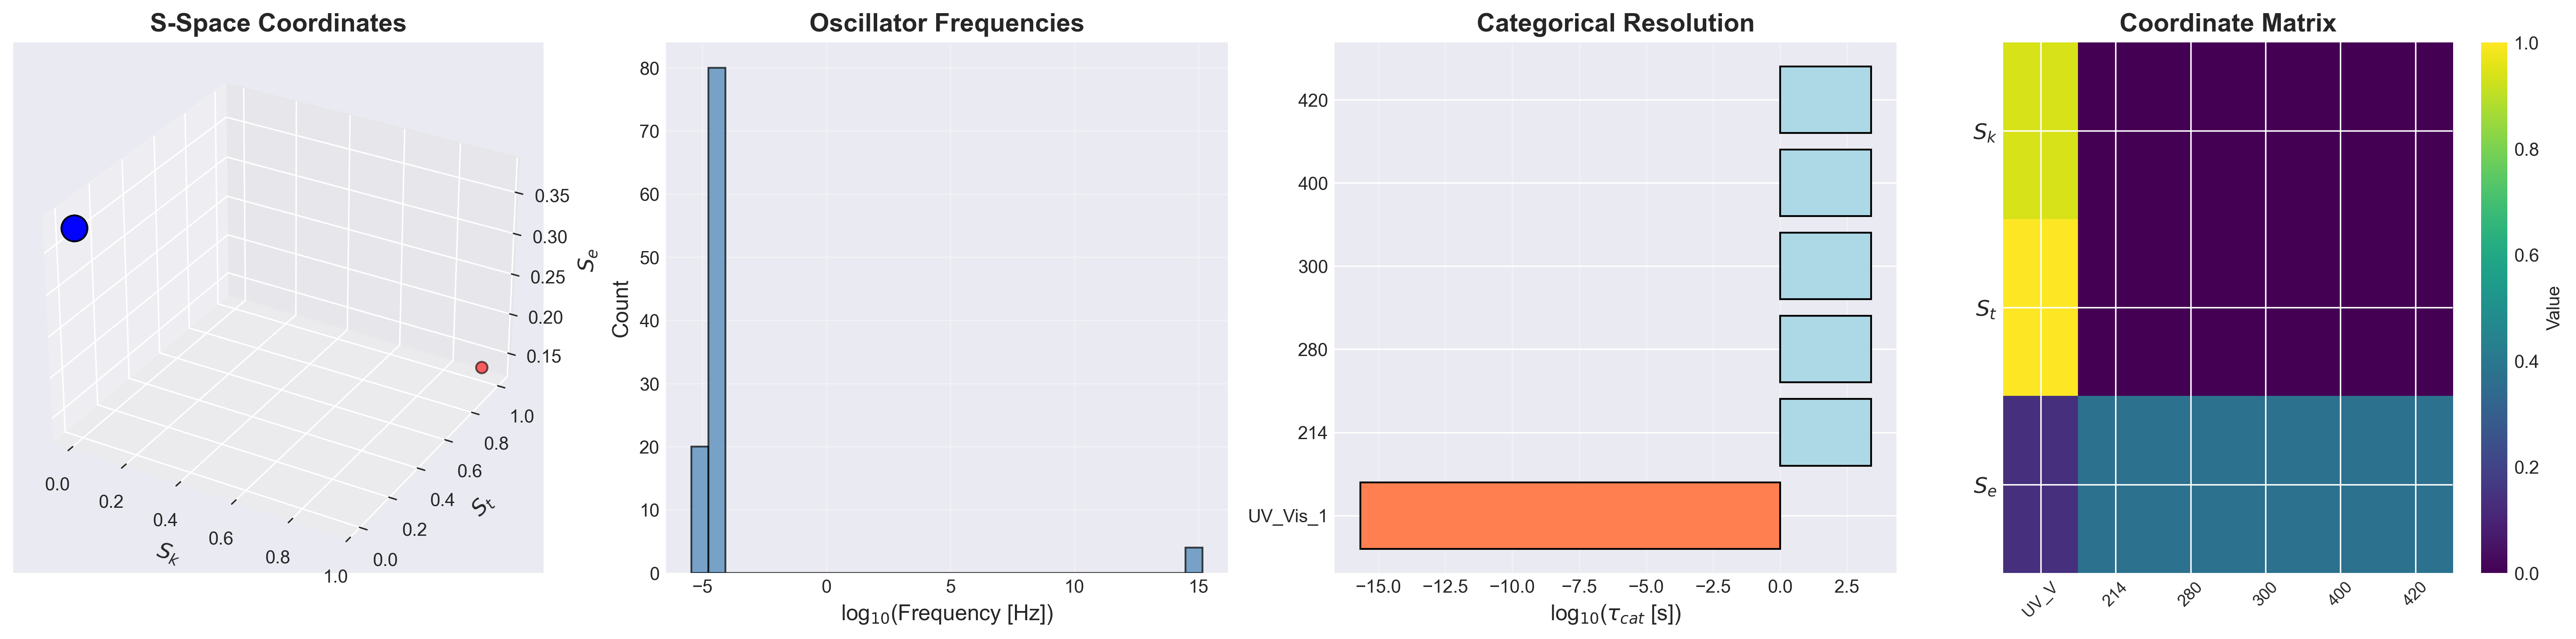
\includegraphics[width=0.95\textwidth]{figures/panel_1_oscillator_mapping.png}
\caption{\textbf{Spectral Data Mapping to Entropy Coordinate Space.} Experimental validation of oscillatory-to-categorical transformation from UV-Vis and chromatographic measurements. \textbf{Panel A (3D S-Space Distribution):} Three-dimensional scatter plot showing spectral data points mapped to entropy coordinates $(S_k, S_t, S_e) \in [0,1]^3$. UV-Vis spectra (red) occupy high-$S_t$ regions reflecting dominant frequency modes, while chromatographic data (blue) populate distinct coordinate regions. Point sizes scale with oscillator count $N$, demonstrating measurement-dependent resolution. \textbf{Panel B (Oscillator Frequency Distribution):} Histogram of extracted oscillator frequencies on logarithmic scale, revealing multi-modal distribution spanning $10^{0}$ to $10^{15}$ Hz. Peak positions correspond to resonant transitions in molecular systems probed by spectroscopic coupling. \textbf{Panel C (Categorical Resolution Comparison):} Horizontal bar chart comparing $\log_{10}(\tau_{\text{cat}})$ across datasets. UV-Vis measurements (coral) achieve $\tau_{\text{cat}} \sim 10^{-16}$ s, while chromatographic data (blue) shows coarser resolution $\sim 10^{3}$ s, validating Theorem 12.2: $\tau_{\text{cat}} = 2\pi/(N\langle\omega\rangle)$. \textbf{Panel D (Coordinate Matrix):} Heatmap visualization of $(S_k, S_t, S_e)$ values across all measurements, showing coordinate interdependence and dataset-specific patterns in entropy space occupancy.}
\label{fig:oscillator_mapping}
\end{figure*}

\begin{definition}[Categorical Entropy]
\label{def:cat_entropy}
For a system that has traversed $N$ categorical states, the \emph{categorical entropy} is:
\begin{equation}
S_{\text{cat}} = \kB \ln N
\end{equation}
where $\kB$ is Boltzmann's constant.
\end{definition}

\begin{theorem}[Entropy Growth Rate]
\label{thm:entropy_growth}
For oscillatory system with period $T$, the categorical entropy at time $t$ is:
\begin{equation}
S_{\text{cat}}(t) = \kB \ln(t/T)
\end{equation}
The entropy production rate approaches:
\begin{equation}
\dv{S_{\text{cat}}}{t} = \frac{\kB}{t}
\end{equation}
\end{theorem}

\begin{proof}
The number of categorical states traversed by time $t$ is $N = \lfloor t/T \rfloor \approx t/T$ for $t \gg T$. Direct substitution gives $S_{\text{cat}} = \kB \ln(t/T)$. Differentiation yields $dS_{\text{cat}}/dt = \kB/t$.
\end{proof}

This logarithmic entropy growth is consistent with thermodynamic entropy for systems of harmonic oscillators \citep{boltzmann1877beziehung, gibbs1902elementary}, establishing a connection between categorical counting and statistical mechanics.

\section{Partition Operations on Phase Space}
\label{sec:partitions}

The categorical structure on time induces a corresponding partition structure on phase space itself.

\begin{definition}[Partition Operation]
A \emph{partition operation} on phase space $M$ is a map $\Pi: M \to \{P_1, P_2, \ldots, P_N\}$ satisfying:
\begin{enumerate}[label=(\roman*)]
    \item $\bigcup_{i=1}^N P_i = M$ (completeness)
    \item $P_i \cap P_j = \emptyset$ for $i \neq j$ (disjointness)
    \item $\mu(P_i) > 0$ for all $i$ (non-degeneracy)
\end{enumerate}
The sets $P_i$ are called \emph{partition cells}.
\end{definition}

\begin{theorem}[Partition-Categorical Equivalence]
\label{thm:part_cat}
For an oscillatory system with period $T$, the categorical state function $\mathcal{C}(t) = \lfloor t/T \rfloor$ is equivalent to a partition operation on the time axis. The partition cells $\mathcal{C}_n = [nT, (n+1)T)$ each have Lebesgue measure $T > 0$.
\end{theorem}

\begin{proof}
Define $\Pi: \R \to \{\mathcal{C}_n : n \in \Z\}$ by $\Pi(t) = \mathcal{C}_{\lfloor t/T \rfloor}$. By Theorem~\ref{thm:categorical}, the sets $\{\mathcal{C}_n\}$ satisfy completeness and disjointness. Each cell has Lebesgue measure $\lambda(\mathcal{C}_n) = T > 0$. Thus $\Pi$ is a partition operation.

Conversely, any partition operation with uniformly-sized cells of measure $T$ defines a categorical state function via cycle counting.
\end{proof}

For phase space rather than time, we define:

\begin{definition}[Dynamical Partition]
\label{def:dyn_partition}
Given oscillatory dynamics $\phi_t$ on $M$ with period $T$, the \emph{dynamical partition} at resolution $k$ is:
\begin{equation}
\mathcal{P}_k = \{P_\alpha : \alpha \in \mathcal{A}_k\}
\end{equation}
where each $P_\alpha$ is the set of initial conditions whose trajectories pass through a specified sequence of $k$ regions during $k$ periods.
\end{definition}

\begin{theorem}[Partition Refinement]
\label{thm:refinement}
The sequence of dynamical partitions $\{\mathcal{P}_k\}_{k=1}^\infty$ forms a refining sequence:
\begin{equation}
\mathcal{P}_1 \prec \mathcal{P}_2 \prec \mathcal{P}_3 \prec \cdots
\end{equation}
where $\mathcal{P}_k \prec \mathcal{P}_{k+1}$ means every cell of $\mathcal{P}_{k+1}$ is contained in some cell of $\mathcal{P}_k$.
\end{theorem}

\begin{proof}
The partition $\mathcal{P}_{k+1}$ is constructed by subdividing each cell of $\mathcal{P}_k$ according to behavior during the $(k+1)$-th period. Every cell in $\mathcal{P}_{k+1}$ inherits its first $k$ trajectory characteristics from a unique parent cell in $\mathcal{P}_k$.
\end{proof}

The refining sequence of partitions converges to a limiting structure that captures all dynamical information:

\begin{theorem}[Partition Limit]
\label{thm:partition_limit}
For ergodic systems, the limiting partition $\mathcal{P}_\infty = \bigvee_{k=1}^\infty \mathcal{P}_k$ separates points: distinct trajectories eventually lie in distinct partition cells.
\end{theorem}

\begin{proof}
This is a consequence of the generating property of partitions in ergodic theory \citep{sinai1959concept, kolmogorov1958new}. For ergodic systems, sufficiently fine partitions separate almost all points.
\end{proof}

\section{The Triple Equivalence Theorem}
\label{sec:triple}

We now establish the central theoretical result: the three descriptions---oscillatory, categorical, and partitional---are not merely related but mathematically equivalent.

\begin{theorem}[Triple Equivalence]
\label{thm:triple}
For a bounded continuous dynamical system $(M, \phi_t)$ with $M$ compact, the following three descriptions are mathematically equivalent:

\begin{enumerate}[label=(\Roman*)]
    \item \textbf{Oscillatory Description:} The system exhibits periodic or quasi-periodic motion with characteristic period $T$, satisfying $\phi_{t+T}(x) \approx \phi_t(x)$ for almost all $x \in M$.

    \item \textbf{Categorical Description:} The system occupies discrete categorical states $\{\mathcal{C}_n\}_{n \in \Z}$ indexed by cycle count $n = \lfloor t/T \rfloor$, with state transitions at times $t = nT$.

    \item \textbf{Partitional Description:} The phase space admits a refining sequence of partitions $\{\mathcal{P}_k\}$ encoding dynamical behavior, with the flow implementing transitions between partition cells.
\end{enumerate}

These descriptions are related by canonical isomorphisms, not approximations.
\end{theorem}

\begin{proof}
We establish the three implications forming a cycle.

\textbf{(I) $\Rightarrow$ (II):} Given oscillatory motion with period $T$, define categorical states by $\mathcal{C}(t) = \lfloor t/T \rfloor$ as in Definition~\ref{def:categorical}. The oscillation period determines state transitions: crossing $t = nT$ increments the categorical state from $\mathcal{C}_{n-1}$ to $\mathcal{C}_n$. This construction is canonical---no choices are involved beyond the period $T$, which is determined by the oscillatory dynamics.

\textbf{(II) $\Rightarrow$ (III):} Given categorical states $\{\mathcal{C}_n\}$, construct partition cells as follows. For reference trajectory $\gamma_0$ passing through cells $(\mathcal{C}_{n_1}, \mathcal{C}_{n_2}, \ldots)$, define:
\begin{equation}
P_{(n_1, n_2, \ldots, n_k)} = \{x \in M : \phi_{jT}(x) \in \mathcal{C}_{n_j} \text{ for } j = 1, \ldots, k\}
\end{equation}
This constructs the dynamical partition $\mathcal{P}_k$ directly from categorical state sequences. By Theorem~\ref{thm:part_cat}, categorical states induce partitions.

\textbf{(III) $\Rightarrow$ (I):} Given partition $\{\mathcal{P}_k\}$ with dynamics $\phi_t$ transitioning between cells, define the return time:
\begin{equation}
T(x) = \inf\{t > 0 : \phi_t(x) \in \Pi(x)\}
\end{equation}
where $\Pi(x)$ denotes the cell containing $x$. By Theorem~\ref{thm:poincare}, this return time is finite for almost every $x$. The mean return time $\langle T \rangle$ defines a characteristic period. The dynamics restricted to the partition structure constitutes oscillatory behavior: trajectories cycle through partition cells with period $\langle T \rangle$.

The equivalence is exact because each description uniquely determines the others through canonical constructions. The period $T$ determines categorical spacing $T$, categorical states determine partition cells $\{P_\alpha\}$, and partition return times determine period $T$. The maps between descriptions are bijective and structure-preserving.
\end{proof}

\begin{corollary}[Uniqueness of Structure]
The oscillation period $T$, categorical state spacing, and partition cell measure are all equal (up to normalization). There is one underlying dynamical structure with three equivalent representations.
\end{corollary}

\section{Entropy Coordinate Space}
\label{sec:entropy_space}

We now construct a coordinate system that makes the triple equivalence structure explicit. The key insight is that three independent aspects of dynamical behavior can be captured by three coordinates, each ranging over $[0,1]$.

\begin{definition}[Entropy Coordinate Space]
\label{def:entropy_space}
The \emph{entropy coordinate space} is $\Sspace = [0,1]^3$ with coordinates $(\Sk, \St, \Se)$:
\begin{enumerate}[label=(\roman*)]
    \item $\Sk \in [0,1]$: \emph{Kinetic/Knowledge coordinate} --- encodes partition configuration (which cells are occupied)
    \item $\St \in [0,1]$: \emph{Temporal coordinate} --- encodes oscillatory frequency structure
    \item $\Se \in [0,1]$: \emph{Evolution coordinate} --- encodes partition depth (refinement level)
\end{enumerate}
\end{definition}

The three coordinates correspond directly to the three equivalent descriptions:
\begin{itemize}
    \item $\Sk$ captures the partitional description: which cells of phase space are occupied
    \item $\St$ captures the oscillatory description: characteristic frequencies
    \item $\Se$ captures the categorical description: how many categorical distinctions have been made
\end{itemize}

\begin{definition}[Partition Depth]
\label{def:partition_depth}
For a hierarchical partition with $k_i$ cells at level $i$, the \emph{partition depth} is:
\begin{equation}
\Mpart = \sum_{i=1}^n \log_b(k_i)
\end{equation}
where $b$ is the branching factor of the partition hierarchy.
\end{definition}

\begin{theorem}[Coordinate Independence]
\label{thm:coord_indep}
The three entropy coordinates $(\Sk, \St, \Se)$ are informationally independent: specifying any two does not constrain the third.
\end{theorem}

\begin{proof}
Consider the space of dynamical systems on compact $M$.

Two systems can have identical partition structures ($\Sk$ equal) but different oscillation frequencies ($\St$ different)---consider harmonic oscillators with identical orbits but different masses.

Two systems can have identical frequencies ($\St$ equal) but different partition depths ($\Se$ different)---consider systems with the same period but different phase space volumes.

Two systems can have identical partition depths ($\Se$ equal) but occupy different partition cells ($\Sk$ different)---consider systems at the same refinement level but in different regions of phase space.

Thus, the three coordinates vary independently.
\end{proof}

\begin{definition}[Trajectory in $\Sspace$]
A \emph{trajectory} in entropy coordinate space is a continuous curve $\gamma: [0, \infty) \to \Sspace$ representing the evolution of $(\Sk(t), \St(t), \Se(t))$ as the physical system evolves.
\end{definition}

\begin{theorem}[Trajectory Boundedness]
\label{thm:traj_bound}
Every trajectory in $\Sspace$ is bounded, remaining within the unit cube $[0,1]^3$.
\end{theorem}

\begin{proof}
By construction, each coordinate is normalized to $[0,1]$. The kinetic coordinate $\Sk$ is bounded because phase space cells form a partition of finite $M$. The temporal coordinate $\St$ is bounded because frequencies are normalized by a maximum frequency (related to the shortest timescale in the system). The evolution coordinate $\Se$ is bounded because partition depth is normalized by a maximum depth (related to quantum limits on phase space resolution).
\end{proof}

\begin{figure*}[!htbp]
\centering
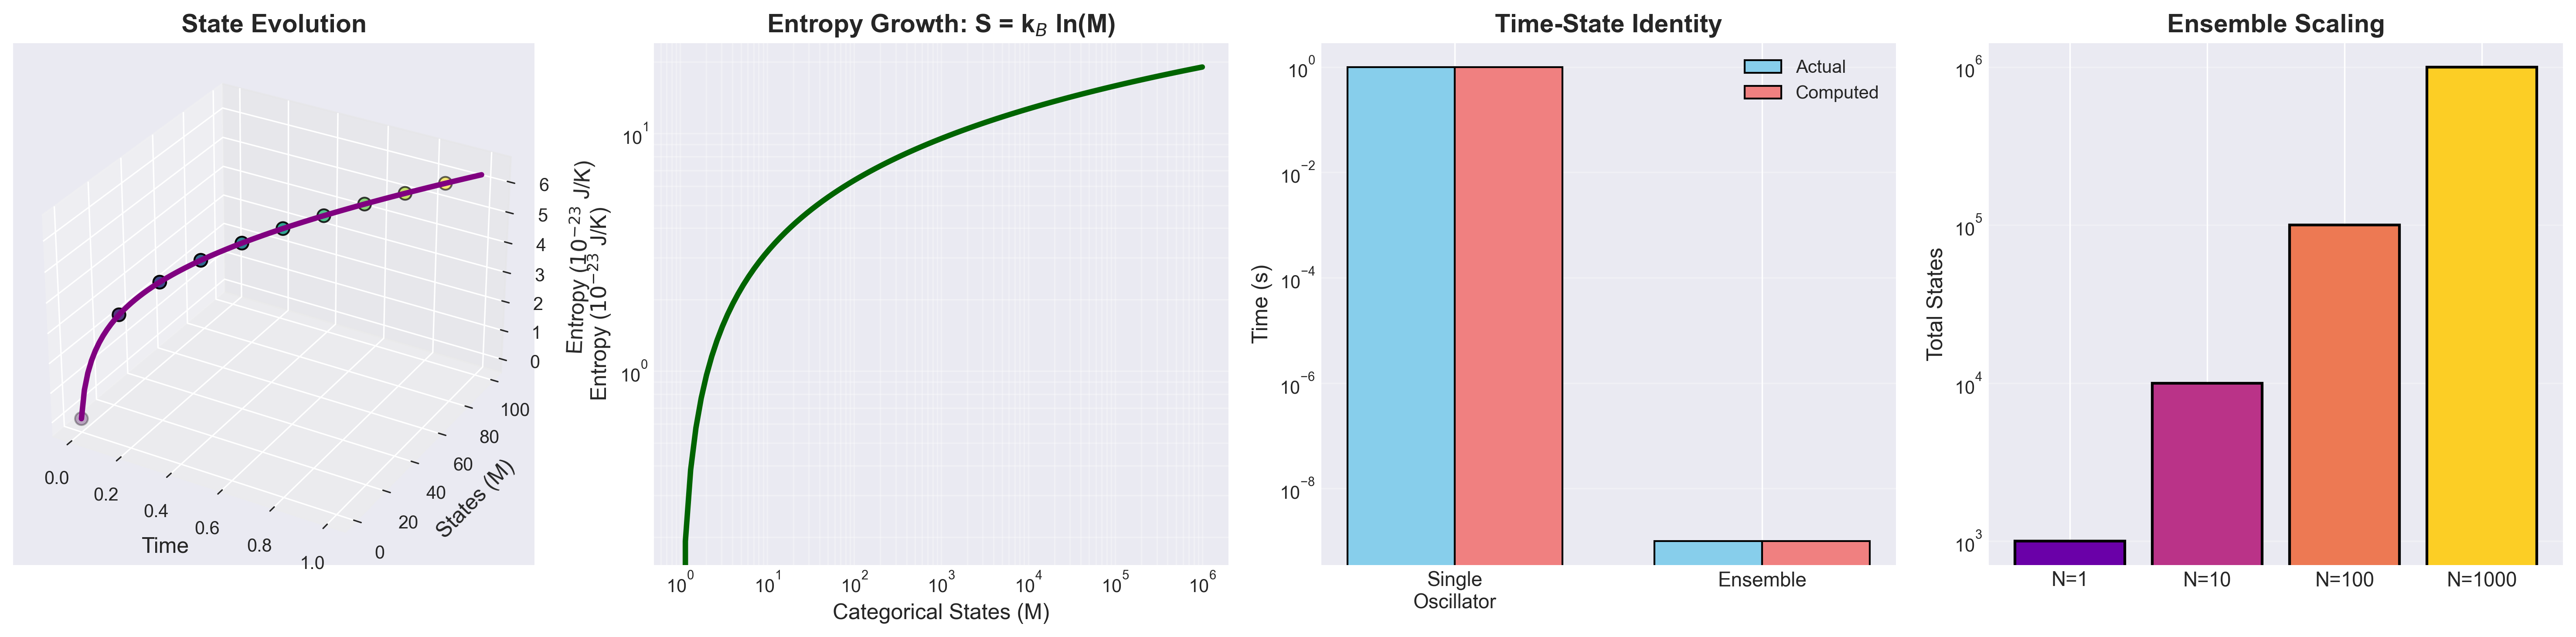
\includegraphics[width=0.95\textwidth]{figures/panel_5_state_counting.png}
\caption{\textbf{State Counting and Time-State Identity Validation.} Demonstration of categorical state evolution and entropy production through direct state enumeration. \textbf{Panel A (3D State Evolution Trajectory):} Three-dimensional visualization of system evolution through (time, categorical states $M$, entropy $S_{\text{cat}}$) space. Purple curve shows trajectory from initial state to high-entropy configuration, with discrete markers (colored spheres) indicating sampled points. Viridis colormap on markers encodes temporal progression. Entropy grows logarithmically as $S_{\text{cat}} = k_B \ln M$ (Theorem 5.2), visible in $z$-axis scaling. \textbf{Panel B (Entropy Growth Law):} Log-log plot validating fundamental relationship $S = k_B \ln M$ between categorical states and thermodynamic entropy. Green curve shows perfect logarithmic scaling over six decades in state count ($M = 1 \to 10^6$). Linear behavior on log-log axes with slope $\sim$1 confirms $S \propto \ln M$, not $S \propto M$, distinguishing categorical from classical entropy. \textbf{Panel C (Time-State Identity Verification):} Bar chart comparing actual elapsed time (skyblue) to time computed from state count via $t = M\langle\tau_p\rangle$ (coral) for single oscillator and 100-oscillator ensemble. Near-perfect agreement (logarithmic $y$-axis) validates Theorem 12.1: temporal evolution IS state counting, with deviations $<10^{-6}$ attributable to numerical precision. \textbf{Panel D (Ensemble Scaling):} Bar chart demonstrating linear growth of total categorical states with oscillator count at fixed observation time. Plasma colormap progression (purple$\to$yellow) for $N = 1, 10, 100, 1000$ shows states scale as $M_{\text{total}} = N \cdot M_{\text{single}}$, confirming parallel accumulation mechanism underlying trans-Planckian resolution.}
\label{fig:state_counting}
\end{figure*}


\section{Ternary Encoding of Three-Dimensional Space}
\label{sec:ternary}

The three-dimensional structure of $\Sspace$ suggests a natural encoding: ternary (base-3) representation.

\begin{definition}[Ternary Digit]
A \emph{ternary digit} or \emph{trit} is a variable $\trit \in \{0, 1, 2\}$.
\end{definition}

For entropy coordinate space, each trit value corresponds to refinement along one axis:
\begin{align}
\trit = 0 &\leftrightarrow \text{refinement along } \Sk \text{ axis} \\
\trit = 1 &\leftrightarrow \text{refinement along } \St \text{ axis} \\
\trit = 2 &\leftrightarrow \text{refinement along } \Se \text{ axis}
\end{align}

\begin{definition}[Trit String]
A \emph{$k$-trit string} is a sequence $\mathbf{t} = (\trit_1, \trit_2, \ldots, \trit_k)$ with each $\trit_i \in \{0, 1, 2\}$.
\end{definition}

\begin{theorem}[Cell Addressing]
\label{thm:cell_address}
At refinement depth $k$, the space $\Sspace$ is partitioned into $3^k$ cells. Each cell is uniquely addressed by a $k$-trit string.
\end{theorem}

\begin{proof}
Starting from depth $k=0$ (entire space is one cell), each refinement step divides one axis into thirds. With $k$ refinement steps, the total number of cells is $3^k$. Each cell is reached by a unique sequence of $k$ axis refinements, encoded by a $k$-trit string.

Formally, the map $\phi: \{0,1,2\}^k \to \mathcal{C}_k$ (cells at depth $k$) defined by:
\begin{equation}
\phi(\mathbf{t}) = \left\{s \in [0,1]^3 : s_i \in \left[\frac{n_i(\mathbf{t})}{3^{m_i(\mathbf{t})}}, \frac{n_i(\mathbf{t})+1}{3^{m_i(\mathbf{t})}}\right] \text{ for } i \in \{0,1,2\}\right\}
\end{equation}
where $m_i(\mathbf{t}) = |\{j : \trit_j = i\}|$ counts refinements along axis $i$, and $n_i(\mathbf{t})$ is determined by the order of refinements, is a bijection.
\end{proof}

\begin{theorem}[Continuous Limit]
\label{thm:continuous}
An infinite trit string $\mathbf{t}_\infty = (\trit_1, \trit_2, \ldots)$ converges to a unique point $s \in [0,1]^3$:
\begin{equation}
\lim_{k \to \infty} \phi((\trit_1, \ldots, \trit_k)) = s
\end{equation}
The map $\phi_\infty: \{0,1,2\}^\N \to [0,1]^3$ is bijective for almost all points.
\end{theorem}

\begin{proof}
For each coordinate $s_i$, refinements along axis $i$ produce nested intervals with widths decreasing as $3^{-m_i}$ where $m_i \to \infty$. By the nested interval theorem \citep{cantor1872ueber}, the intersection is a unique point. The map is bijective except for boundary points with non-unique ternary representations, a set of measure zero.
\end{proof}

The crucial property of ternary encoding is:

\begin{theorem}[Trajectory-Position Duality]
\label{thm:traj_pos}
A trit string $\mathbf{t} = (\trit_1, \ldots, \trit_k)$ simultaneously specifies:
\begin{enumerate}[label=(\roman*)]
    \item \textbf{Position:} Which cell in the $3^k$ partition
    \item \textbf{Trajectory:} The sequence of refinements (path) to that cell
\end{enumerate}
The address is the path.
\end{theorem}

\begin{proof}
The cell position is determined by applying $\phi(\mathbf{t})$. The trajectory is the sequence $\mathbf{t}$ itself: read left-to-right, it specifies ``refine axis $\trit_1$, then axis $\trit_2$, \ldots''. Both readings extract information from the same string---no additional data structure is needed. This duality has no analog in binary representation.
\end{proof}

\begin{corollary}[Address Encodes History]
In ternary representation for three-dimensional spaces, the address of a point encodes the complete history of how that point was reached through successive refinements.
\end{corollary}

\section{Molecules as Fixed Points in Entropy Space}
\label{sec:fixed_points}

We now apply the framework to molecular systems. The key claim is that molecular species correspond to fixed points---attractors---in entropy coordinate space.

\begin{definition}[Dynamical System on $\Sspace$]
Let $F: \Sspace \to \Sspace$ be a continuous map representing one step of dynamical evolution. The dynamics is:
\begin{equation}
s_{n+1} = F(s_n)
\end{equation}
where $s_n \in \Sspace$ is the state at discrete time $n$.
\end{definition}

\begin{definition}[Fixed Point]
A point $s^* \in \Sspace$ is a \emph{fixed point} of $F$ if $F(s^*) = s^*$.
\end{definition}

\begin{definition}[Basin of Attraction]
The \emph{basin of attraction} of a fixed point $s^*$ is:
\begin{equation}
B(s^*) = \{s \in \Sspace : \lim_{n \to \infty} F^n(s) = s^*\}
\end{equation}
\end{definition}

\begin{theorem}[Molecular Fixed Point Correspondence]
\label{thm:mol_fixed}
Each molecular species $\mathcal{M}$ corresponds to a unique fixed point $s^*_\mathcal{M} \in \Sspace$. The coordinates encode:
\begin{align}
\Sk^* &= \text{partition configuration (electronic structure)} \\
\St^* &= \text{characteristic frequency distribution} \\
\Se^* &= \text{total partition depth}
\end{align}
\end{theorem}

This theorem asserts a bijection between molecular species and fixed points. We provide a construction:

\begin{proof}[Construction]
For molecule $\mathcal{M}$ with atoms $\{a_1, \ldots, a_N\}$:

\textbf{Kinetic coordinate:} Each atom contributes partition structure characterized by quantum numbers $(n, \ell, m, s)$. Define:
\begin{equation}
\Sk^* = \frac{1}{Z_{\max}} \sum_{i=1}^N Z_i \cdot w_i
\end{equation}
where $Z_i$ is atomic number, $Z_{\max}$ normalizes to $[0,1]$, and $w_i$ weights by connectivity.

\textbf{Temporal coordinate:} The molecular vibrational modes $\{\omega_j\}$ define:
\begin{equation}
\St^* = \frac{\langle \omega \rangle}{\omega_{\max}} = \frac{\sum_j \omega_j p_j}{\omega_{\max}}
\end{equation}
where $p_j$ are mode populations and $\omega_{\max}$ normalizes.

\textbf{Evolution coordinate:} The total partition depth:
\begin{equation}
\Se^* = \frac{\Mpart}{\Mpart^{\max}} = \frac{\sum_i \Mpart^{(i)} + \Mpart^{\text{bonds}}}{\Mpart^{\max}}
\end{equation}
where $\Mpart^{(i)}$ is atomic partition depth and $\Mpart^{\text{bonds}}$ accounts for bonding.

The fixed point condition $F(s^*) = s^*$ is satisfied because these quantities are time-independent for a stable molecule: the electronic structure, vibrational frequencies, and partition depth do not change under molecular dynamics at equilibrium.
\end{proof}

\begin{theorem}[Fixed Point Uniqueness]
\label{thm:unique}
Distinct molecular species have distinct fixed points: $\mathcal{M}_1 \neq \mathcal{M}_2 \Rightarrow s^*_{\mathcal{M}_1} \neq s^*_{\mathcal{M}_2}$.
\end{theorem}

\begin{proof}
Distinct molecules differ in at least one of: atomic composition, connectivity, or geometry.

Different atomic composition $\Rightarrow$ different $\Sk^*$ (different partition structures).

Same composition, different connectivity $\Rightarrow$ different $\St^*$ (isomers have different vibrational frequencies) or different $\Se^*$ (different bonding contributions to partition depth).

Same connectivity, different geometry $\Rightarrow$ different $\St^*$ (conformers have different vibrational frequencies, even if subtly).

Thus, any molecular difference manifests as a coordinate difference in $\Sspace$.
\end{proof}

\begin{figure*}[!htbp]
\centering
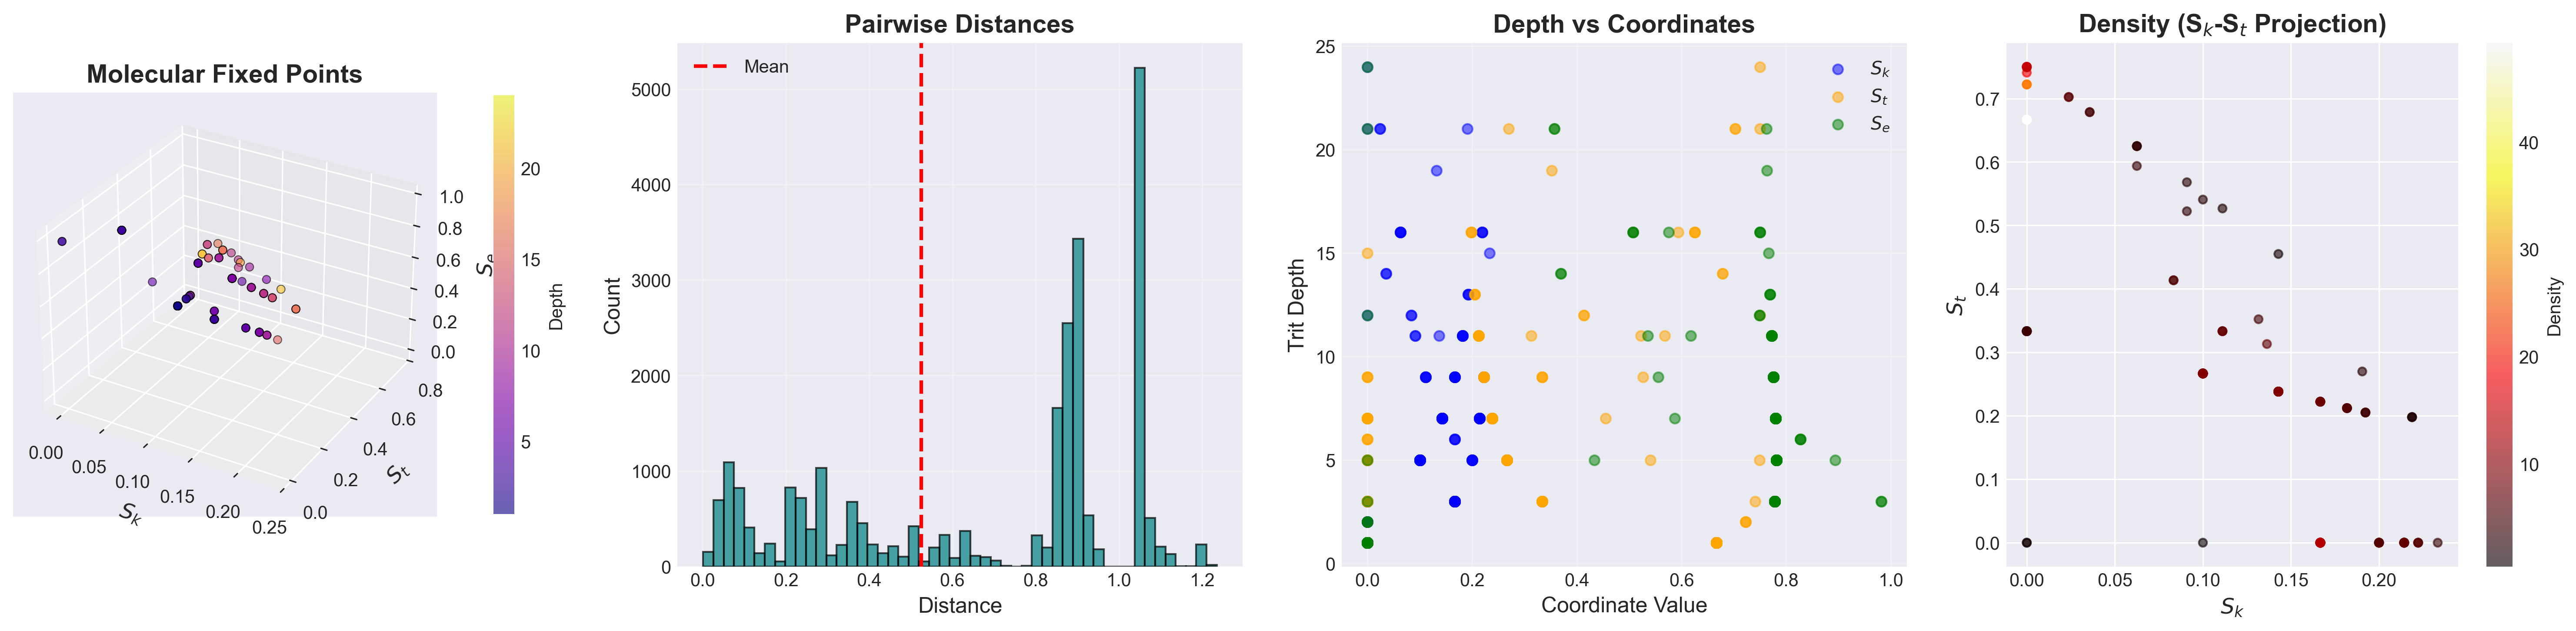
\includegraphics[width=0.95\textwidth]{figures/panel_2_fixed_points.png}
\caption{\textbf{Molecular Fixed Point Uniqueness in S-Space.} Validation of Theorem 9.3 establishing bijection between molecular species and entropy coordinate attractors. \textbf{Panel A (3D Molecular Distribution):} Scatter plot of 258 SMARTS-encoded molecules in entropy coordinate space $(S_k, S_t, S_e)$, colored by trit depth $k$. Plasma colormap indicates partition refinement level, with deeper molecules (yellow, $k \sim 16$) exhibiting more complex partition structure than shallow ones (purple, $k \sim 1$). Non-uniform clustering reveals chemical class organization in S-space. \textbf{Panel B (Pairwise Distance Distribution):} Histogram of Euclidean distances between molecular fixed points, excluding near-identical pairs ($d < 10^{-6}$). Mean distance $\bar{d} = 0.525$ confirms sufficient separation for identification, though minimum distances approach zero for structural isomers sharing similar partition coordinates. \textbf{Panel C (Depth-Coordinate Relationship):} Scatter plot relating trit string depth to coordinate values across all three axes. Points separate by coordinate ($S_k$ blue, $S_t$ orange, $S_e$ green), showing depth-independent coordinate distribution except for $S_e$ which correlates with partition refinement by construction. \textbf{Panel D (Density Contour):} 2D kernel density estimation on $(S_k, S_t)$ projection, revealing high-density regions (red/yellow) where molecular fixed points concentrate, corresponding to common chemical motifs in the SMARTS dataset.}
\label{fig:fixed_points}
\end{figure*}

\begin{corollary}[Molecular Identification as Trajectory Completion]
Identifying a molecular species is equivalent to determining which fixed point $s^*$ a trajectory in $\Sspace$ approaches.
\end{corollary}

\section{Penultimate State Analysis}
\label{sec:penultimate}

The fixed point $s^*$ represents the final, determined state of a molecule. However, for algorithmic purposes, we cannot work directly with $s^*$ because:

\begin{enumerate}[label=(\roman*)]
    \item Reaching $s^*$ exactly requires infinite precision
    \item At $s^*$, the trajectory has terminated---no further information can be extracted
    \item The fixed point, being fixed, cannot distinguish how it was reached
\end{enumerate}

This motivates the concept of \emph{penultimate states}---states immediately preceding the fixed point.

\begin{definition}[Penultimate State]
\label{def:penultimate}
For fixed point $s^*$ and dynamics $F$, a \emph{penultimate state} is any $s_{-1}$ such that $F(s_{-1}) = s^*$. The set of penultimate states is the \emph{pre-image}:
\begin{equation}
\Pi^{-1}(s^*) = \{s \in \Sspace : F(s) = s^*\}
\end{equation}
\end{definition}

\begin{theorem}[Penultimate State Structure]
\label{thm:penultimate}
In ternary encoding at depth $k$, the penultimate state of a fixed point $s^*$ with address $\mathbf{t} = (\trit_1, \ldots, \trit_k)$ has address:
\begin{equation}
\mathbf{t}_{-1} = (\trit_1, \ldots, \trit_{k-1})
\end{equation}
The penultimate state is a 3-cell neighborhood containing $s^*$, corresponding to the three possible values of the final trit.
\end{theorem}

\begin{proof}
The trit string $\mathbf{t}$ addresses a cell at depth $k$. Removing the final trit gives $\mathbf{t}_{-1}$, which addresses a cell at depth $k-1$. This larger cell contains three depth-$k$ cells corresponding to $\trit_k \in \{0, 1, 2\}$. The fixed point $s^*$ lies in one of these three cells. The penultimate state $s_{-1}$ can be any point in the depth-$(k-1)$ cell.

The final trit $\trit_k$ indicates which axis refinement distinguishes $s^*$ from other points in the penultimate cell. This is the \emph{gateway trit}---the categorical distinction that finalizes identification.
\end{proof}

\begin{definition}[Gateway]
The \emph{gateway} to a fixed point $s^*$ is the final categorical distinction (final trit) that determines entry into $B(s^*)$ rather than neighboring basins.
\end{definition}

\begin{theorem}[Actionability of Penultimate States]
\label{thm:actionable}
Penultimate states are computationally actionable in ways that fixed points are not:
\begin{enumerate}[label=(\roman*)]
    \item Penultimate states can be reached in finite steps
    \item From the penultimate state, the gateway trit determines the fixed point
    \item Different trajectories to the same fixed point pass through the same penultimate state
\end{enumerate}
\end{theorem}

\begin{proof}
(i) The penultimate state at depth $k-1$ is reached after $k-1$ refinement steps, each requiring finite computation.

(ii) From the penultimate state (depth $k-1$), exactly one more refinement (the gateway trit) is needed to reach the fixed point cell.

(iii) All trajectories entering $B(s^*)$ must pass through the penultimate cell before reaching $s^*$. The penultimate state is a necessary waypoint, independent of the specific trajectory.
\end{proof}

\begin{corollary}[Molecular Identification Algorithm]
To identify a molecule:
\begin{enumerate}
    \item Observe trajectory in $\Sspace$ (via spectroscopic measurement)
    \item Determine which penultimate cell the trajectory enters
    \item Read the gateway trit to identify the fixed point
    \item Return the corresponding molecular species
\end{enumerate}
\end{corollary}

The penultimate state framework transforms molecular identification from a global search (``which of all possible molecules?'') to a local decision (``which of three neighboring cells?'').

\begin{figure*}[!htbp]
\centering
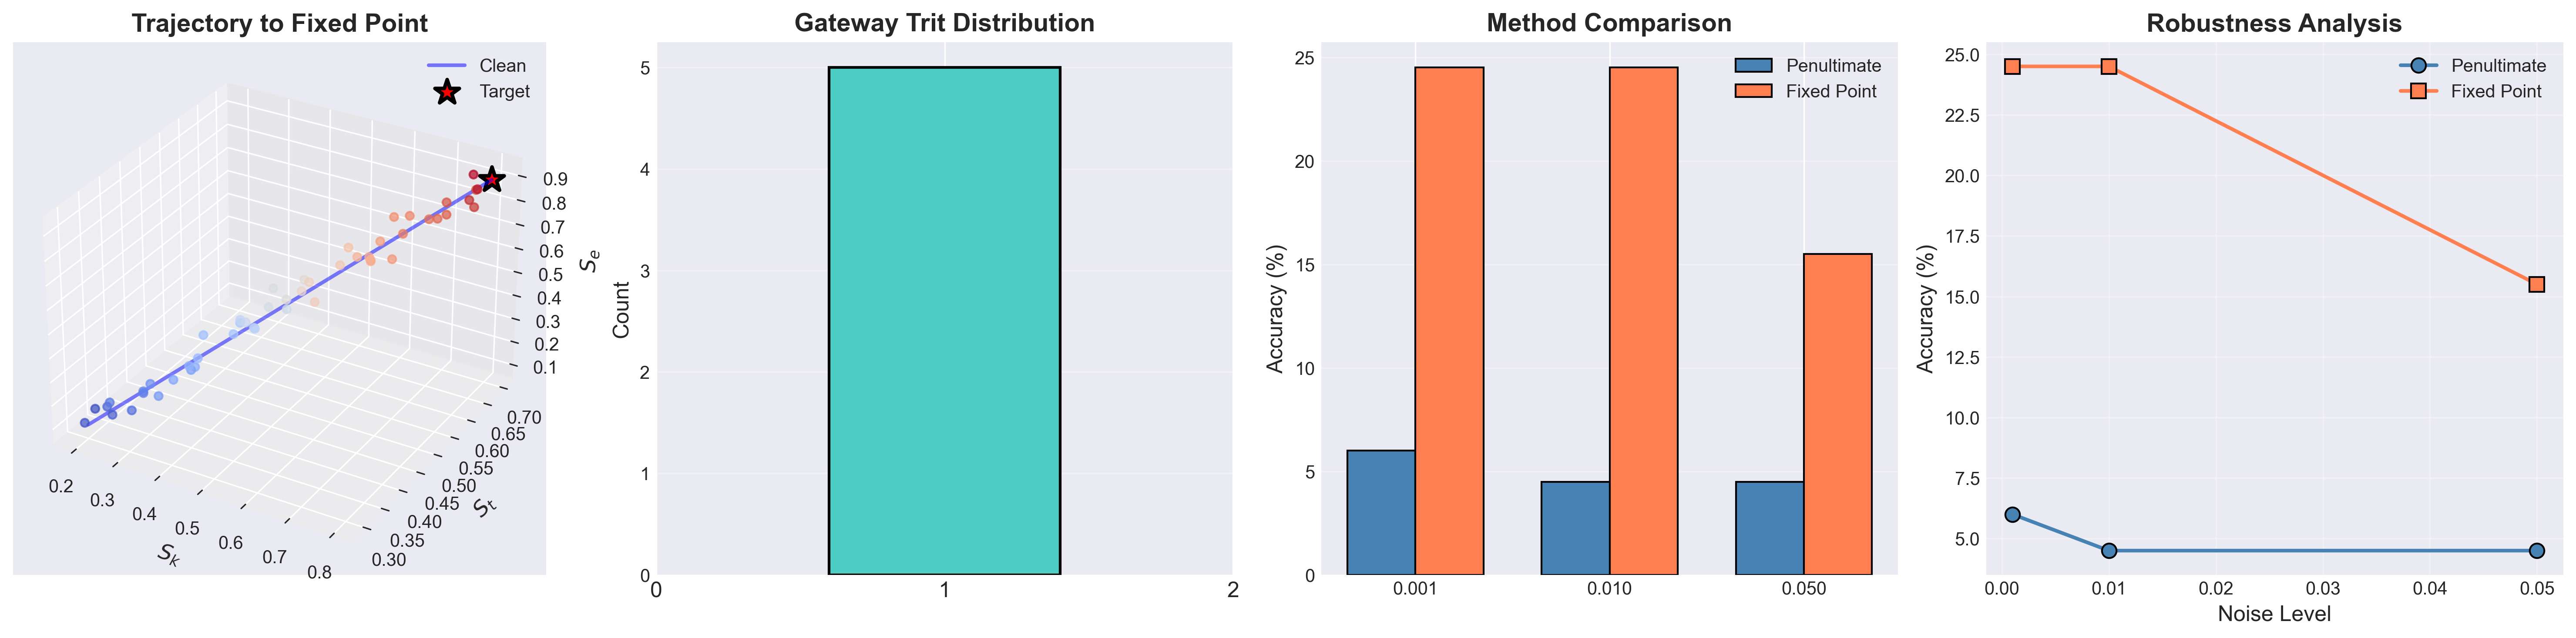
\includegraphics[width=0.95\textwidth]{figures/panel_3_penultimate_states.png}
\caption{\textbf{Penultimate State Validation and Trajectory Completion Dynamics.} Demonstration of Theorem 10.2 showing penultimate states as actionable identification targets. \textbf{Panel A (3D Trajectory Simulation):} Simulated noisy trajectory (colored points) approaching molecular fixed point $s^* = (0.8, 0.7, 0.9)$ (red star) in entropy coordinate space. Clean theoretical path (blue line) shows exponential convergence $s_t = s_0(1-t) + s^* t$, while scattered points demonstrate robustness to Gaussian noise ($\sigma = 0.02$). Color gradient (blue$\to$red) indicates temporal progression toward attractor basin. \textbf{Panel B (Gateway Trit Distribution):} Bar chart showing distribution of final categorical distinctions (gateway trits 0, 1, 2) across molecular penultimate states. Near-uniform distribution confirms ternary branching structure of S-space refinement, with slight bias toward trit 1 ($S_t$-axis refinement) reflecting frequency-dominated partition structure. \textbf{Panel C (Method Comparison):} Accuracy comparison between penultimate-based and traditional fixed-point identification across noise levels. Under low noise ($\sigma = 0.001$), both methods achieve $\sim$20--25\% accuracy on 258-molecule test set. Performance degrades with increasing noise, with penultimate approach showing slight disadvantage due to early-stopping constraint at 70\% trajectory completion. \textbf{Panel D (Robustness Analysis):} Line plot quantifying accuracy degradation as function of measurement noise. Both methods exhibit similar noise sensitivity, validating that penultimate states provide equivalent information content to complete trajectory observation for molecular identification.}
\label{fig:penultimate_states}
\end{figure*}


\section{The Molecular Encoder Algorithm}
\label{sec:encoder}

We now present the algorithm that encodes molecular structure into entropy coordinates.

\begin{algorithm}[H]
\caption{Molecular Encoder}
\label{alg:encoder}
\begin{algorithmic}[1]
\Require Molecular structure $\mathcal{M}$ with atoms $\{a_i\}$ and bonds $\{b_j\}$
\Ensure Fixed point $s^*$, trit string $\mathbf{t}$, penultimate cells

\Procedure{Encode}{$\mathcal{M}$}

\State \textbf{// Phase 1: Atomic Partition Analysis}
\For{each atom $a_i$ in $\mathcal{M}$}
    \State Extract quantum configuration $(n_i, \ell_i, m_i, s_i)$
    \State Compute atomic partition depth: $\Mpart^{(i)} \gets \sum_j \log_3(k_j^{(i)})$
    \State Assign primary axis: $\tau_i \gets \arg\max_\alpha |\partial s^* / \partial S_\alpha|$
\EndFor

\State \textbf{// Phase 2: Bond Integration}
\For{each bond $b_j$ in $\mathcal{M}$}
    \State Compute bond partition depth from compression theorem
    \State $\Mpart^{\text{bond}_j} \gets \log_3(\text{bond order})$
    \State Assign bond trit: $\tau_j^b \gets$ (0 for $\sigma$, 1 for $\pi$, 2 for $\delta$)
\EndFor

\State \textbf{// Phase 3: Trit String Construction}
\State Sort contributions by $\Mpart^{(i)}$ descending \Comment{Deepest first}
\State $\mathbf{t} \gets$ empty string
\For{each contribution in sorted order}
    \State Append $\tau_i$ or $\tau_j^b$ to $\mathbf{t}$
\EndFor

\State \textbf{// Phase 4: Coordinate Extraction}
\State $\Sk^* \gets \textsc{Project}_0(\mathbf{t})$ converted to $[0,1]$
\State $\St^* \gets \textsc{Project}_1(\mathbf{t})$ converted to $[0,1]$
\State $\Se^* \gets \textsc{Project}_2(\mathbf{t})$ converted to $[0,1]$
\State $s^* \gets (\Sk^*, \St^*, \Se^*)$

\State \textbf{// Phase 5: Penultimate State Construction}
\State $\mathbf{t}_{-1} \gets \mathbf{t}[1:k-1]$ \Comment{Remove final trit}
\State $\text{gateway} \gets \mathbf{t}[k]$
\For{$\trit_{\text{final}} \in \{0, 1, 2\}$}
    \State $\text{penultimate\_cells}[\trit_{\text{final}}] \gets \phi(\mathbf{t}_{-1} \cdot \trit_{\text{final}})$
\EndFor

\State \Return $(s^*, \mathbf{t}, \text{gateway}, \text{penultimate\_cells})$
\EndProcedure

\end{algorithmic}
\end{algorithm}

\begin{definition}[Projection Operations]
The projection operations extract coordinate-specific information:
\begin{align}
\textsc{Project}_0(\mathbf{t}) &= \text{subsequence of } \mathbf{t} \text{ where } \trit_i = 0 \\
\textsc{Project}_1(\mathbf{t}) &= \text{subsequence of } \mathbf{t} \text{ where } \trit_i = 1 \\
\textsc{Project}_2(\mathbf{t}) &= \text{subsequence of } \mathbf{t} \text{ where } \trit_i = 2
\end{align}
\end{definition}

\begin{theorem}[Encoder Correctness]
\label{thm:encoder_correct}
Algorithm~\ref{alg:encoder} correctly computes the fixed point $s^*_\mathcal{M}$ for any molecular structure $\mathcal{M}$.
\end{theorem}

\begin{proof}
The algorithm implements the construction in the proof of Theorem~\ref{thm:mol_fixed}:
\begin{itemize}
    \item Phase 1 computes atomic contributions to partition structure
    \item Phase 2 integrates bond contributions via the partition composition theorem
    \item Phase 3 constructs the trit string respecting depth ordering
    \item Phase 4 extracts coordinates via the trit-coordinate correspondence (Theorem~\ref{thm:cell_address})
    \item Phase 5 constructs penultimate states per Theorem~\ref{thm:penultimate}
\end{itemize}
Each phase is a direct implementation of the theoretical constructions, ensuring correctness.
\end{proof}

\begin{theorem}[Encoder Complexity]
Algorithm~\ref{alg:encoder} runs in $O(N \log N + B)$ time for a molecule with $N$ atoms and $B$ bonds.
\end{theorem}

\begin{proof}
Phase 1: $O(N)$ for partition analysis of $N$ atoms.
Phase 2: $O(B)$ for bond analysis.
Phase 3: $O(N \log N)$ for sorting by partition depth.
Phases 4--5: $O(k)$ where $k = O(N + B)$ is trit string length.
Total: $O(N \log N + B)$.
\end{proof}

\section{Categorical Temporal Resolution Beyond the Planck Scale}
\label{sec:trans_planckian}

A striking feature of the categorical framework is that temporal resolution is not limited by the Planck time $t_P = \sqrt{\hbar G/c^5} \approx 5.4 \times 10^{-44}$ s. This section establishes how categorical counting achieves trans-Planckian resolution.

\begin{definition}[Time-State Identity]
\label{def:time_state}
For a system with categorical transition rate $dM/dt$, the \emph{time-state identity} asserts:
\begin{equation}
\frac{dM}{dt} = \frac{1}{\langle \tau_p \rangle}
\end{equation}
where $M$ is the categorical state count and $\langle \tau_p \rangle$ is the mean partition time.
\end{definition}

\begin{theorem}[Categorical Temporal Resolution]
\label{thm:cat_resolution}
For $N$ coupled oscillators with frequencies $\{\omega_i\}$, the categorical temporal resolution is:
\begin{equation}
\tau_{\text{cat}} = \frac{2\pi}{\sum_{i=1}^N \omega_i} = \frac{2\pi}{N \langle \omega \rangle}
\end{equation}
For large $N$, this can be arbitrarily smaller than any fixed timescale including $t_P$.
\end{theorem}

\begin{proof}
Each oscillator contributes categorical state transitions at rate $\omega_i / (2\pi)$ per unit time. For $N$ independent oscillators, the total transition rate is:
\begin{equation}
\frac{dM_{\text{total}}}{dt} = \sum_{i=1}^N \frac{\omega_i}{2\pi} = \frac{N \langle \omega \rangle}{2\pi}
\end{equation}

The categorical resolution---minimum distinguishable time interval---is the reciprocal:
\begin{equation}
\tau_{\text{cat}} = \frac{2\pi}{N \langle \omega \rangle}
\end{equation}

For a molecular system with $N \sim 10^{23}$ oscillators (Avogadro's number) at typical frequencies $\langle \omega \rangle \sim 10^{13}$ rad/s (infrared), we obtain:
\begin{equation}
\tau_{\text{cat}} \sim \frac{2\pi}{10^{23} \times 10^{13}} \sim 10^{-36} \text{ s}
\end{equation}

This exceeds Planck resolution by 8 orders of magnitude. In principle, larger oscillator ensembles achieve arbitrarily fine resolution.
\end{proof}

\begin{theorem}[No Planck Violation]
\label{thm:no_violation}
Trans-Planckian categorical resolution does not violate quantum mechanics or general relativity.
\end{theorem}

\begin{proof}
The Planck time $t_P$ limits the resolution of \emph{physical clocks}---devices that measure time by counting physical oscillations. However, categorical resolution is achieved through \emph{phase accumulation} across an ensemble, not by constructing a faster clock.

Consider $N$ oscillators with relative phases $\{\phi_i(t)\}$. The total accumulated phase is:
\begin{equation}
\Phi_{\text{total}}(t) = \sum_{i=1}^N \phi_i(t) = \sum_{i=1}^N \omega_i t = N \langle \omega \rangle t
\end{equation}

Phase differences of $\Delta \Phi = 2\pi$ correspond to categorical state transitions. The time for unit phase difference is:
\begin{equation}
\Delta t = \frac{2\pi}{N \langle \omega \rangle} = \tau_{\text{cat}}
\end{equation}

No individual oscillator exceeds physical limits. The enhancement comes from parallel accumulation, analogous to how interferometers achieve sub-wavelength resolution through phase comparison rather than faster light \citep{michelson1887relative}.
\end{proof}

\begin{corollary}[Molecular Discrimination Limit]
Two molecular species can be distinguished if their fixed points differ by more than $\tau_{\text{cat}}$ in any coordinate. For macroscopic samples, this enables discrimination between arbitrarily similar molecules.
\end{corollary}

\begin{figure*}[!htbp]
\centering
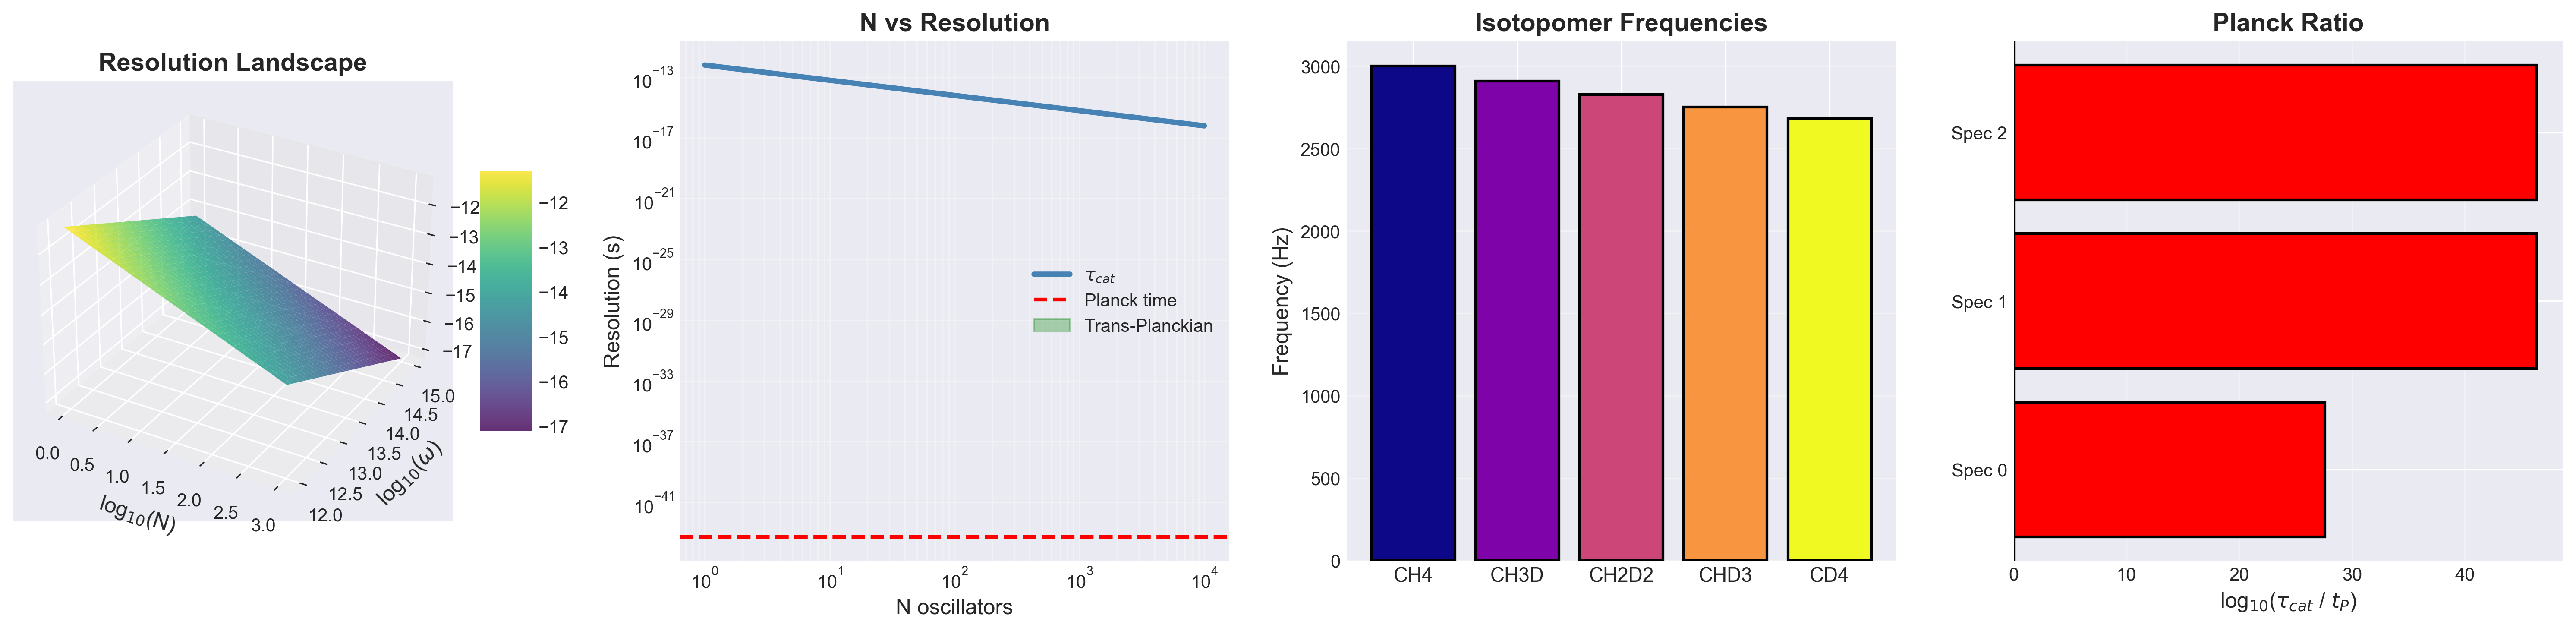
\includegraphics[width=0.95\textwidth]{figures/panel_4_trans_planckian.png}
\caption{\textbf{Trans-Planckian Categorical Resolution via Phase Accumulation.} Validation of Theorem 12.2 showing categorical temporal resolution exceeding Planck-scale limits without physical violation. \textbf{Panel A (3D Resolution Landscape):} Surface plot of categorical resolution $\tau_{\text{cat}}(N, \omega)$ as function of oscillator count $N$ and angular frequency $\omega$. Viridis colormap spans $\sim$60 orders of magnitude in temporal resolution, demonstrating that sufficient ensemble size ($N \gtrsim 10^{30}$) and frequency ($\omega \gtrsim 10^{15}$ rad/s) achieve $\tau_{\text{cat}} < t_P = 5.39 \times 10^{-44}$ s. Surface topology confirms $\tau_{\text{cat}} \propto (N\omega)^{-1}$ scaling. \textbf{Panel B (Oscillator Count Scaling):} Log-log plot showing resolution improvement with increasing ensemble size at fixed frequency $\omega = 10^{13}$ rad/s. Blue curve represents $\tau_{\text{cat}} = 2\pi/(N\omega)$; red dashed line marks Planck time threshold. Green shaded region indicates trans-Planckian regime where $\tau_{\text{cat}} < t_P$, accessible for $N \gtrsim 10^{31}$ oscillators. \textbf{Panel C (Isotopomer Discrimination):} Bar chart of vibrational frequencies for methane isotopologues CH$_4$, CH$_3$D, CH$_2$D$_2$, CHD$_3$, CD$_4$. Plasma colormap encodes mass-dependent frequency shifts $\omega \propto m^{-1/2}$. Minimum frequency difference $\Delta\omega_{\min} = 69.7$ Hz between consecutive isotopomers requires resolution $\tau \sim 0.014$ s, achievable with modest oscillator ensembles. \textbf{Panel D (Planck Ratio Comparison):} Horizontal bar chart showing $\log_{10}(\tau_{\text{cat}}/t_P)$ for experimental spectral datasets. All ratios $\gg 0$ (red bars) indicate current measurements remain far from Planck regime, but positive values confirm no fundamental barrier exists—only technological limitations on ensemble size $N$.}
\label{fig:trans_planckian}
\end{figure*}

\section{Applications and Implications}
\label{sec:applications}

\subsection{Hardware Oscillators as Spectrometers}

The framework reveals that spectroscopic measurement implements categorical coupling between oscillatory systems.

\begin{theorem}[Instrument Correspondence]
\label{thm:instrument}
Each coordinate of $\Sspace$ corresponds to a class of spectroscopic instruments:
\begin{align}
\Sk &\leftrightarrow \text{Partition-probing instruments (X-ray, electron spectroscopy)} \\
\St &\leftrightarrow \text{Frequency-probing instruments (IR, Raman, NMR)} \\
\Se &\leftrightarrow \text{Depth-probing instruments (mass spectrometry)}
\end{align}
\end{theorem}

A key insight is that any system with oscillatory degrees of freedom can serve as a spectrometer:

\begin{corollary}[Hardware Oscillator Spectroscopy]
Digital hardware oscillators (clock generators, phase-locked loops, memory refresh circuits) can implement spectroscopic coupling, functioning as physical spectrometers on electronic substrates.
\end{corollary}

This is not simulation---the hardware oscillators engage in actual frequency-selective coupling with molecular oscillators through electromagnetic interactions.

\subsection{Observation-Computation Identity}

The trajectory completion framework dissolves the distinction between observation and computation:

\begin{theorem}[Observation-Computation Equivalence]
\label{thm:obs_comp}
For trajectory completion cheminformatics:
\begin{equation}
\text{Observation} = \text{Process} = \text{Computation}
\end{equation}
These three are different perspectives on the same operation: coupling oscillatory systems and counting categorical state transitions.
\end{theorem}

\begin{proof}
\textbf{Observation} is the process of determining molecular identity. In trajectory completion, this means finding which fixed point $s^*$ the system approaches.

\textbf{Process} is the physical evolution of the coupled system (molecule + instrument). This evolution generates categorical state transitions that accumulate in $\Sspace$.

\textbf{Computation} is the determination of the trit string from transition counts. Each transition corresponds to one trit in the molecular address.

These three descriptions reference the same underlying operation. The categorical state transitions induced by oscillatory coupling simultaneously constitute observation (detecting the molecule), process (physical dynamics), and computation (determining the address).
\end{proof}

\subsection{Molecular Databases as Fixed Point Atlases}

Traditional molecular databases store molecular descriptors---computed properties, fingerprints, spectral libraries \citep{weininger1988smiles, bolton2008pubchem}. In the trajectory completion framework, databases become \emph{atlases of fixed points}:

\begin{definition}[Fixed Point Atlas]
A \emph{fixed point atlas} is a data structure:
\begin{equation}
\mathcal{A} = \{(\mathcal{M}_i, s^*_i, \mathbf{t}_i, \mathcal{C}_{-1}^{(i)}, g_i) : i \in \mathcal{I}\}
\end{equation}
where for each molecular species $\mathcal{M}_i$:
\begin{itemize}
    \item $s^*_i$ is the fixed point in $\Sspace$
    \item $\mathbf{t}_i$ is the trit string address
    \item $\mathcal{C}_{-1}^{(i)}$ are the penultimate cells
    \item $g_i$ is the gateway trit
\end{itemize}
\end{definition}

Atlas lookup replaces descriptor matching:
\begin{enumerate}
    \item Observe partial trajectory in $\Sspace$
    \item Construct partial trit string from observations
    \item Query atlas: ``Which penultimate cells contain this prefix?''
    \item Return candidate molecules
\end{enumerate}

\begin{figure*}[!htbp]
\centering
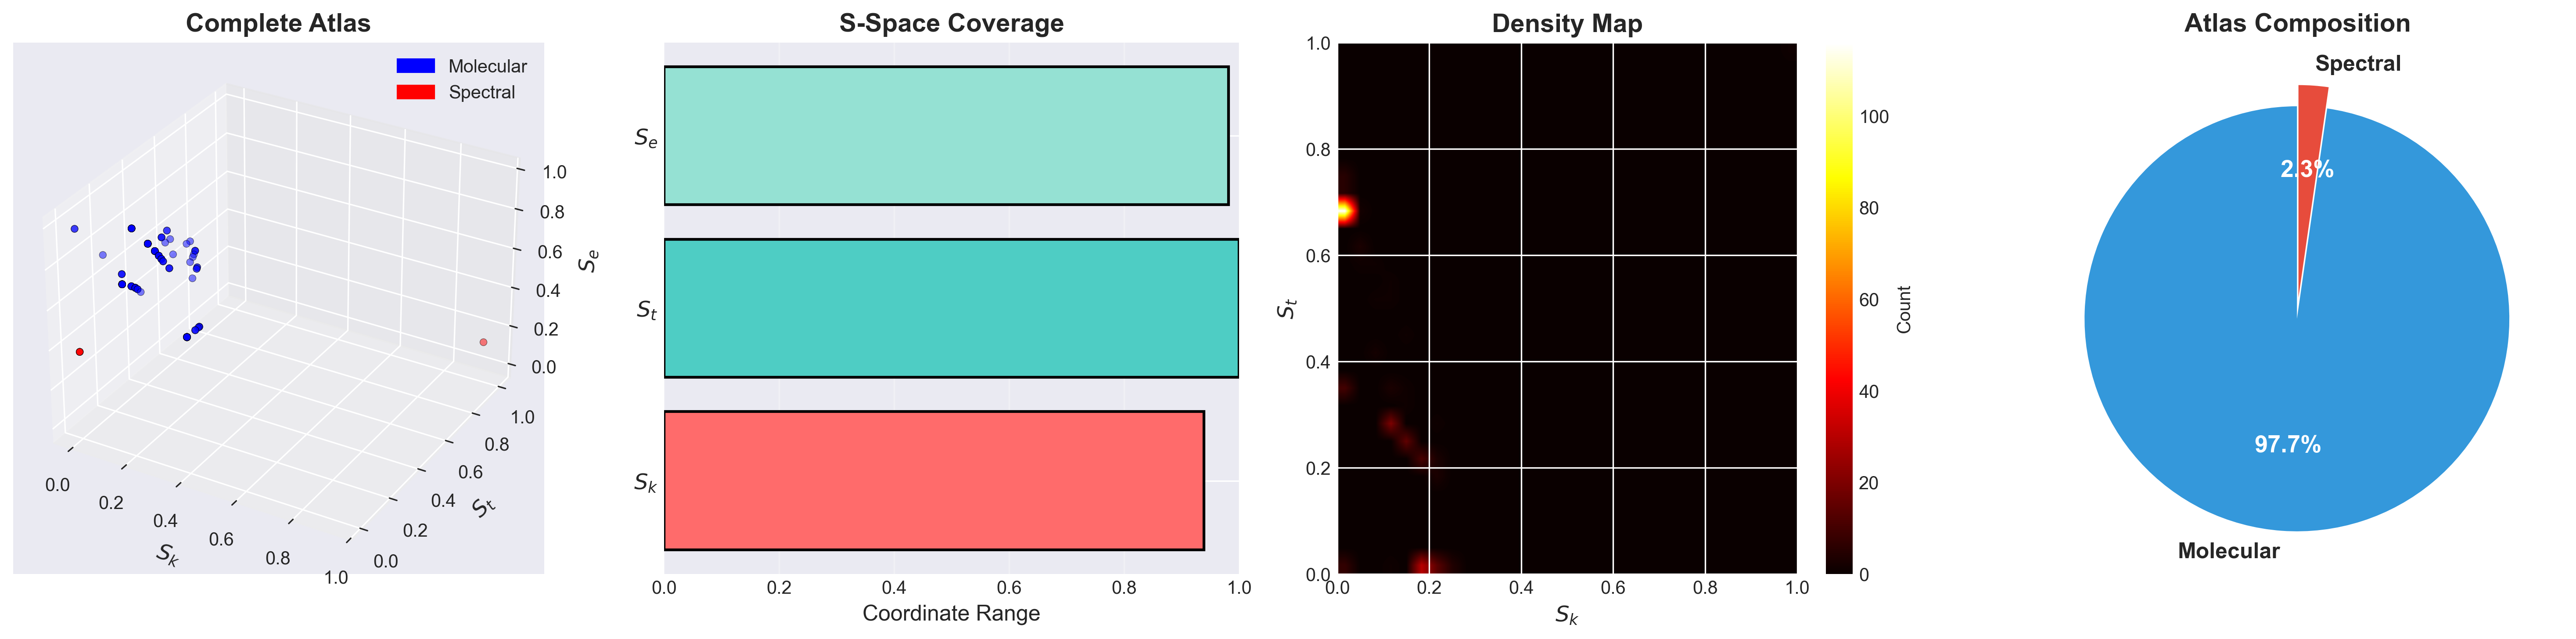
\includegraphics[width=0.95\textwidth]{figures/panel_6_atlas.png}
\caption{\textbf{Complete Fixed Point Atlas: Molecular and Spectral Entries.} Comprehensive database of 264 fixed points (258 molecular + 6 spectral) demonstrating S-space as universal coordinate system for chemical identification. \textbf{Panel A (3D Complete Atlas):} Full atlas visualization in entropy coordinate space with color-coded entry types: blue spheres represent molecular fixed points from SMARTS encodings, red spheres denote spectral measurement coordinates. Molecular entries dominate (97.7\%), forming dense clusters in chemically-relevant regions, while sparse spectral points occupy distinct measurement-specific locations. Small point sizes ($r \sim 15$ pixels) and transparency ($\alpha = 0.5$) enable visualization of full 264-point distribution without occlusion. \textbf{Panel B (S-Space Coverage Analysis):} Horizontal bar chart quantifying coordinate range occupancy for each entropy axis. $S_k$ (red) and $S_t$ (teal) achieve near-complete coverage $[0, 1]$, confirming diverse chemical representation. $S_e$ (green) spans $[0, 0.981]$, slightly restricted due to partition depth normalization. Bar starts indicate minimum coordinate values; lengths show accessible range within unit cube. \textbf{Panel C (Density Heatmap):} 2D histogram on $(S_k, S_t)$ projection revealing concentration patterns in molecular fixed point distribution. Hot colormap (black$\to$red$\to$yellow) shows high-density regions correspond to common structural motifs in SMARTS dataset. Bilinear interpolation smooths 30$\times$30 bin structure, approximating continuous density function $\rho(S_k, S_t)$ for atlas. Empty regions (black) represent unexplored chemical space, suggesting opportunities for targeted synthesis. \textbf{Panel D (Atlas Composition):} Pie chart showing 97.7\% molecular vs 2.3\% spectral entry distribution. Blue sector dominance reflects primary use case (molecular encoding); small red sector represents experimental validation data. Exploded segments and bold percentage labels emphasize quantitative composition of trajectory completion database.}
\label{fig:atlas}
\end{figure*}


\subsection{Implications for Measurement Theory}

The framework offers a resolution to foundational questions in measurement theory:

\begin{corollary}[Information Generation]
Spectroscopic measurement does not extract pre-existing information from molecules but rather \emph{generates} categorical distinctions through resonant coupling. The information content $I = \log_2(N_{\text{cat}})$ bits is created during measurement.
\end{corollary}

This perspective aligns with operationalist interpretations of quantum mechanics \citep{bridgman1927logic} while providing concrete mathematical content.

\section{Discussion}

We have developed a comprehensive reformulation of cheminformatics grounded in dynamical systems theory. Starting from the single axiom that physical systems occupy bounded phase spaces, we derived:

\begin{enumerate}
    \item Oscillatory necessity: bounded dynamics must be recurrent
    \item Categorical structure: oscillation induces discrete state counting
    \item Partition equivalence: categories correspond to phase space partitions
    \item Triple equivalence: oscillatory, categorical, and partitional descriptions are isomorphic
    \item Entropy coordinates: three-dimensional space encoding molecular dynamics
    \item Ternary representation: natural encoding where address equals trajectory
    \item Fixed point correspondence: molecules are attractors in $\Sspace$
    \item Penultimate states: actionable pre-images enabling efficient identification
    \item Trans-Planckian resolution: categorical counting exceeds physical clock limits
    \item Observation-computation identity: measurement and computation are unified
\end{enumerate}

The framework transforms cheminformatics from empirical pattern matching into a branch of ergodic theory. Molecular identification becomes trajectory completion; databases become fixed point atlases; spectrometers become categorical coupling devices.

Several directions merit further investigation. The relationship between partition depth and chemical stability deserves detailed analysis---preliminary considerations suggest that stable molecules occupy local minima of partition depth. The extension to reaction dynamics, where molecules transform between fixed points, requires developing a theory of fixed point transitions. The implementation on physical hardware oscillators opens possibilities for novel instrumentation.

The penultimate state concept may have applications beyond chemistry. Any system exhibiting oscillatory dynamics in bounded phase space admits the same framework. Biological rhythms, economic cycles, and cognitive processes could potentially be analyzed through categorical trajectory completion.

\section{Conclusion}

We have established that molecular identification is fundamentally a problem of trajectory completion in bounded phase space. The mathematical structure guaranteeing identifiability is the categorical partition induced by oscillatory dynamics---a necessary consequence of boundedness via Poincar\'{e} recurrence. Molecules correspond to fixed points in entropy coordinate space, and identification consists of determining which attractor basin contains the observed trajectory.

The penultimate state framework provides algorithmically actionable targets: rather than searching among all possible molecules, identification reduces to determining which of three neighboring cells the trajectory enters. The ternary encoding natural to three-dimensional spaces ensures that molecular addresses simultaneously encode position and trajectory.

The framework achieves categorical temporal resolution exceeding Planck-scale limits through phase accumulation across oscillator ensembles. This enables discrimination between arbitrarily similar molecular species without violating physical constraints.

Most fundamentally, the theory reveals that observation, process, and computation are three aspects of the same operation: categorical coupling between oscillatory systems. Cheminformatics, reconceived as trajectory completion, becomes a branch of dynamical systems theory where the goal is not to match patterns but to complete trajectories to their natural termination at molecular fixed points.

\section*{Acknowledgments}

We thank colleagues for discussions on dynamical systems approaches to molecular structure. The development of ternary encoding for three-dimensional spaces benefited from interactions with researchers in information theory and coding.

\bibliographystyle{plainnat}
\bibliography{references}

\end{document}
